Consider Hamiltonian $H = H_0 + \lambda V$ and the Schrieffer-Wolff transformation is defined as
\begin{equation*}
	H = e^{\lambda S} \hat{H} e^{-\lambda S},
\end{equation*}
with $S\D = -S$ and $S$ chosen, such that the linear term $\lambda V$ is eliminated
\begin{equation*}
	e^{\lambda \hat{S}} \hat{H} e^{-\lambda \hat{S}} = \hat{H}_0 + \O(\lambda^2).
\end{equation*}

Using the Campbell-Baker-Hausdorff formula \textbf{(a)}
\begin{equation*}
	\hat{H}' = e^{\lambda \hat{S}} \hat{H} e^{-\lambda \hat{S}} = \hat{H} + [\lambda \hat{S}, \hat{H}] + \tfrac{1}{2} [\lambda \hat{S}, [\lambda \hat{S}, \hat{H}]] + \ldots,
\end{equation*}
substituting the Hamiltonian 
\begin{equation*}
	\hat{H} = \hat{H}_0 + \lambda \hat{V} + [\lambda \hat{S}, \hat{H}_0 + \lambda \hat{V}] = \ldots + \lambda\left(
		 \hat{V} + \hat{S} \hat{H}_0 - \hat{H}_0 \hat{S}
	\right),
\end{equation*}
we get the condition \textbf{(b)}
\begin{equation}
	[\hat{S}, \hat{H}_0] + \hat{V} = 0.
\end{equation}
Using this condition we can simplify the series expansion \textbf{(c)}
\begin{equation}
	\hat{H}' = \hat{H}_0 + \tfrac{\lambda^2}{2} [\hat{S}, \hat{V}] + \O(\lambda^3).
\end{equation}


Now let’s apply this formalism to the Jaynes-Cummings Hamiltonian in the large detuning limit:
\begin{equation*}
	\hat{H} = \omega \hat{a}\D \hat{a} - \frac{\omega_0}{2} \hat{\sigma}_z + g\left(\hat{a}\D \hat{\sigma}^- + \hat{a} \hat{\sigma}^+\right).
\end{equation*}
The coupling term $\hat{V} = g (\hat{a}\D \hat{\sigma}^- + \hat{a} \hat{\sigma}^+)$ couples the states $\ket{g,n+1}$ and $\ket{e,n}$ with  \textbf{(d)}
\begin{equation*}
	\bk{g,n+1}[\hat{H}]{g,n+1} = \omega n + \omega,
	\hspace{5 mm} 
	\bk{e,n}[\hat{H}]{e,n} = \omega n + \omega_0,
	\hspace{0.5cm} \Rightarrow \hspace{0.5cm}
	\Delta = \omega - \omega_0.
\end{equation*}
To find $\hat{S}$ we could start with ansatz $\hat{S} = \alpha \hat{a}\D \hat{\sigma}^- - \bar{\alpha} \hat{a} \hat{\sigma}^+$ and find \textbf{(e)}
\begin{equation*}
	\alpha = -\frac{1}{\Delta}.
\end{equation*}
That leads to the effective Hamiltonian \textbf{(f)}
\begin{equation*}
	\hat{H}' = \left(\omega + \tfrac{g^2}{\Delta} \hat{\sigma}_z\right) \hat{a}\D \hat{a} - \tfrac{1}{2}\left(\omega_0 + \tfrac{g^2}{\Delta}\right)\hat{\sigma}_z.
\end{equation*}




\begin{figure}[h]
    \centering
    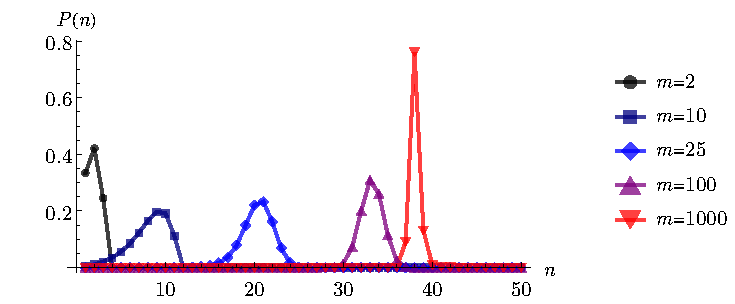
\includegraphics[width=0.7\textwidth]{imgs/QH6.pdf}
    \caption{\textbf{(6.4.c)} The distribution $P_n(m)$ as a function of $n$ for $gt = \tfrac{1}{2}$}
    \label{fig:3}
\end{figure}